\chapter{Experimental Results And Performance Analysis}


\section{Experimental Results}
Web and mobile platform has been tested in our project. Different scenarios were applied with these tests and there was 0.02 percent error observed.

\section{Performance Analysis}

Performance tests were calculated with Apache JMeter tool which makes HTTP request simultaneously depending upon call number that we give. We monitored the CPU and RAM percentage at the server side by using HTOP tool. We called home page with GET method up to for 200 users simultaneously. Different outputs for different number of calls is shown below. HTTP calls loop count is 10 and time interval between loop counts is 10 seconds.

One of the example HTTP call is shown in Figure 
\ref{fig:exampleCall}.

\begin{figure}[!htbp]
\centering
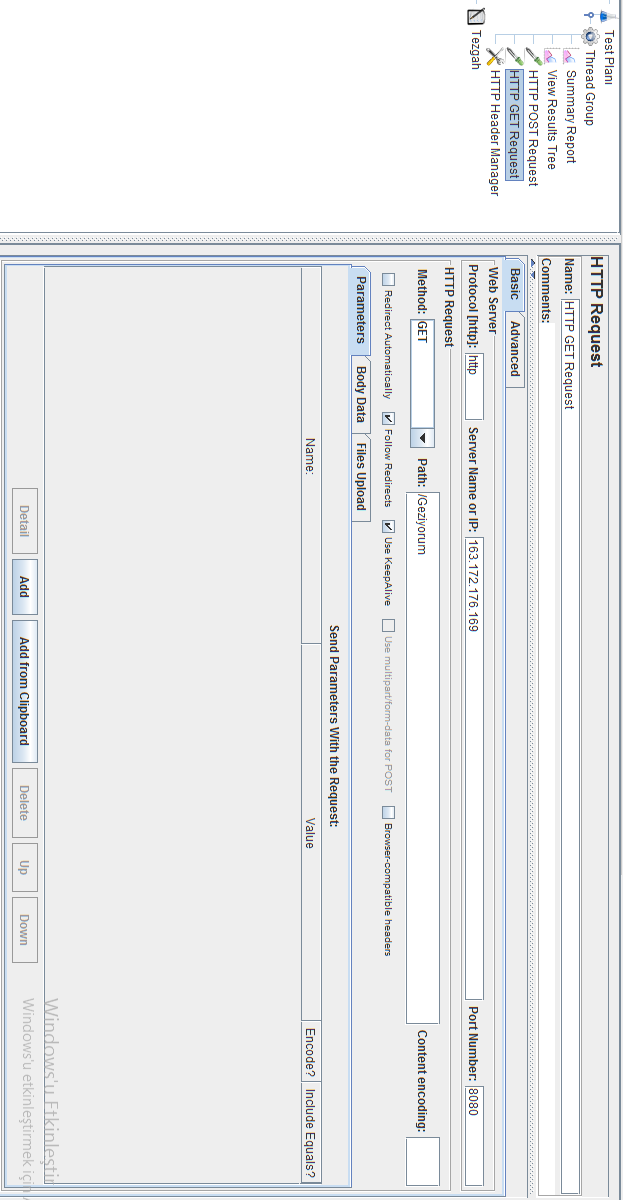
\includegraphics[width=\textwidth]{projectChapters/images/exampleCall.png}
\caption{When server is idle position}
\label{fig:exampleCall}
\end{figure}

\newpage

Server's idle performance is shown in Figure 
\ref{fig:serveridle}.

\begin{figure}[!htbp]
\centering
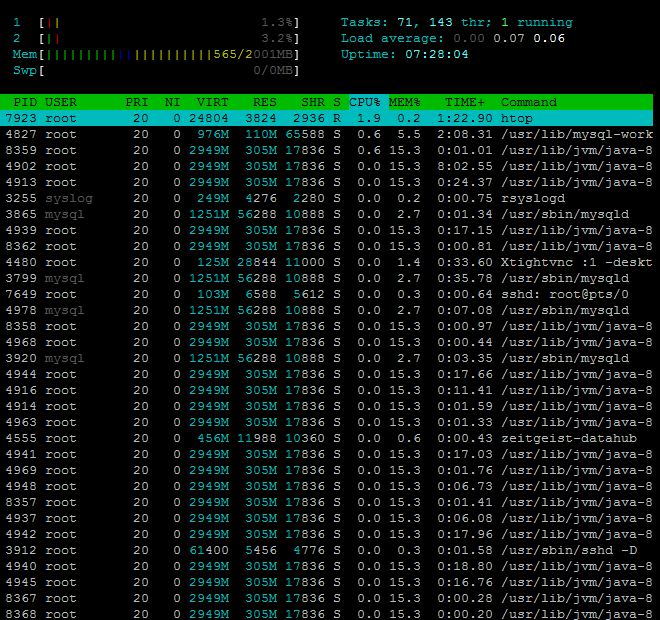
\includegraphics[width=\textwidth]{projectChapters/images/serveridle.png}
\caption{When server is idle position}
\label{fig:serveridle}
\end{figure}

\newpage

When server's performance 30 user simultaneous GET call is shown Figure
\ref{fig:30users}.

\begin{figure}[!htbp]
\centering
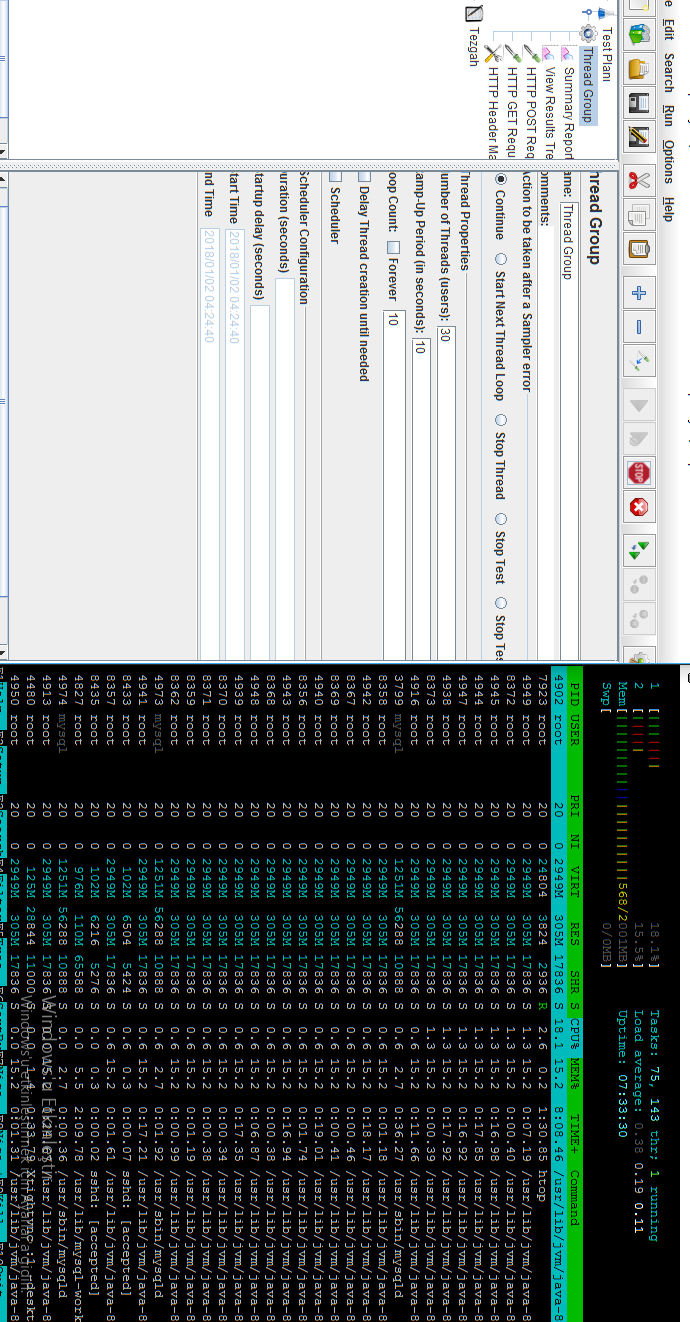
\includegraphics[width=\textwidth]{projectChapters/images/30users.png}
\caption{Server 30 GET HTTP calls simultaneously}
\label{fig:30users}
\end{figure}

\newpage

When server's performance 100 user simultaneous GET call is shown Figure
\ref{fig:100users}.

\begin{figure}[!htbp]
\centering
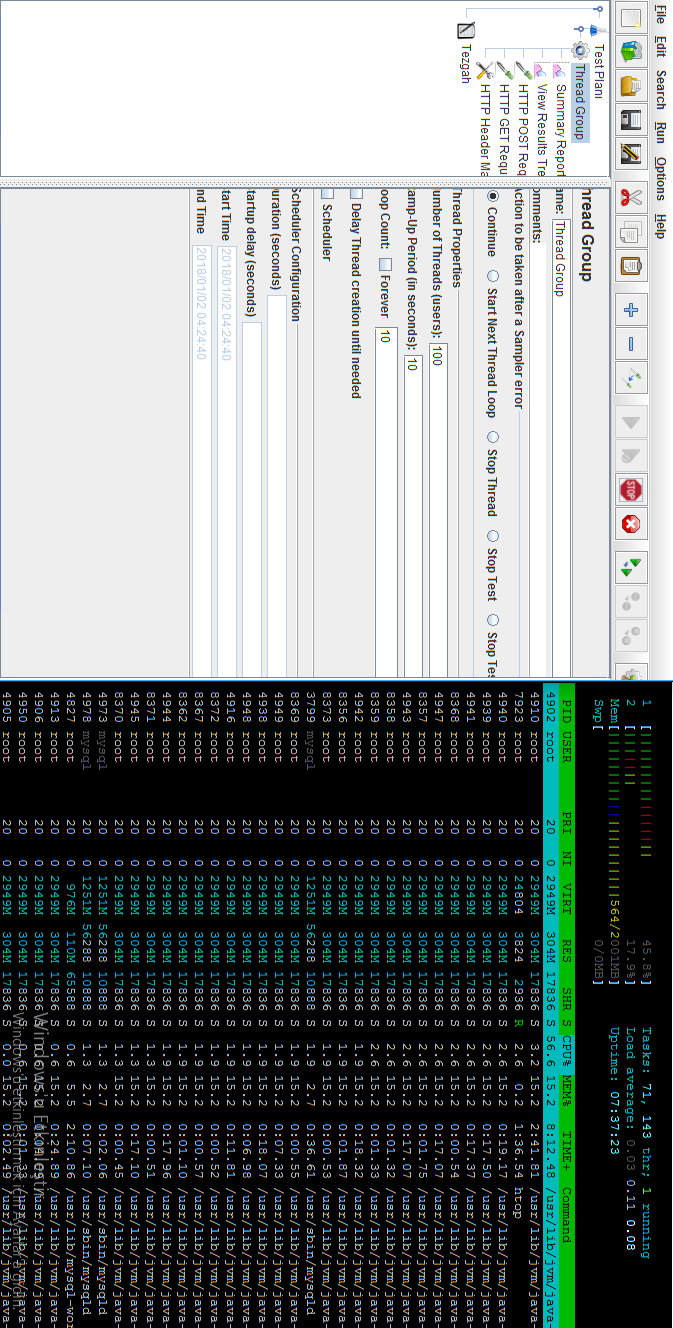
\includegraphics[width=\textwidth]{projectChapters/images/100users.png}
\caption{Server 100 GET HTTP calls simultaneously}
\label{fig:100users}
\end{figure}

\newpage

When server's performance 130 user simultaneous GET and POST call is shown Figure
\ref{fig:130users}.

\begin{figure}[!htbp]
\centering
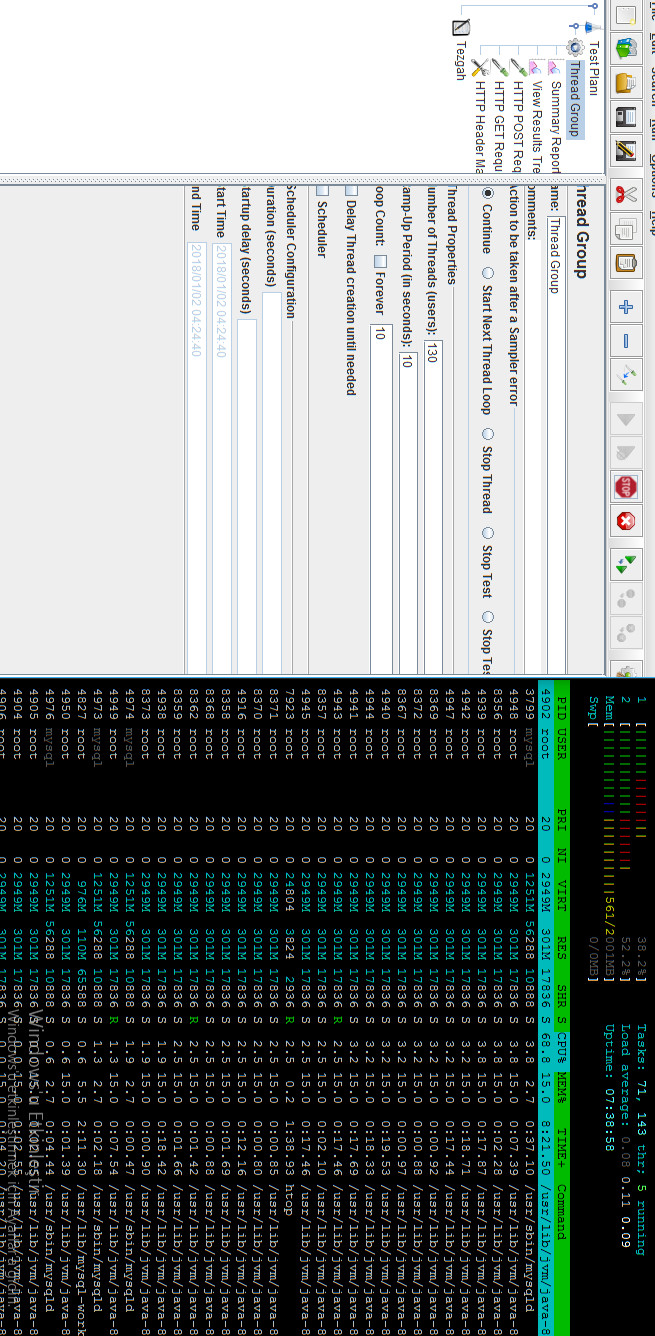
\includegraphics[width=\textwidth]{projectChapters/images/130users.png}
\caption{Server 130 GET and POST HTTP calls simultaneously}
\label{fig:130users}
\end{figure}

\newpage


When server's performance 180 user simultaneous GET and two POST call is shown Figure
\ref{fig:180user}.

\begin{figure}[!htbp]
\centering
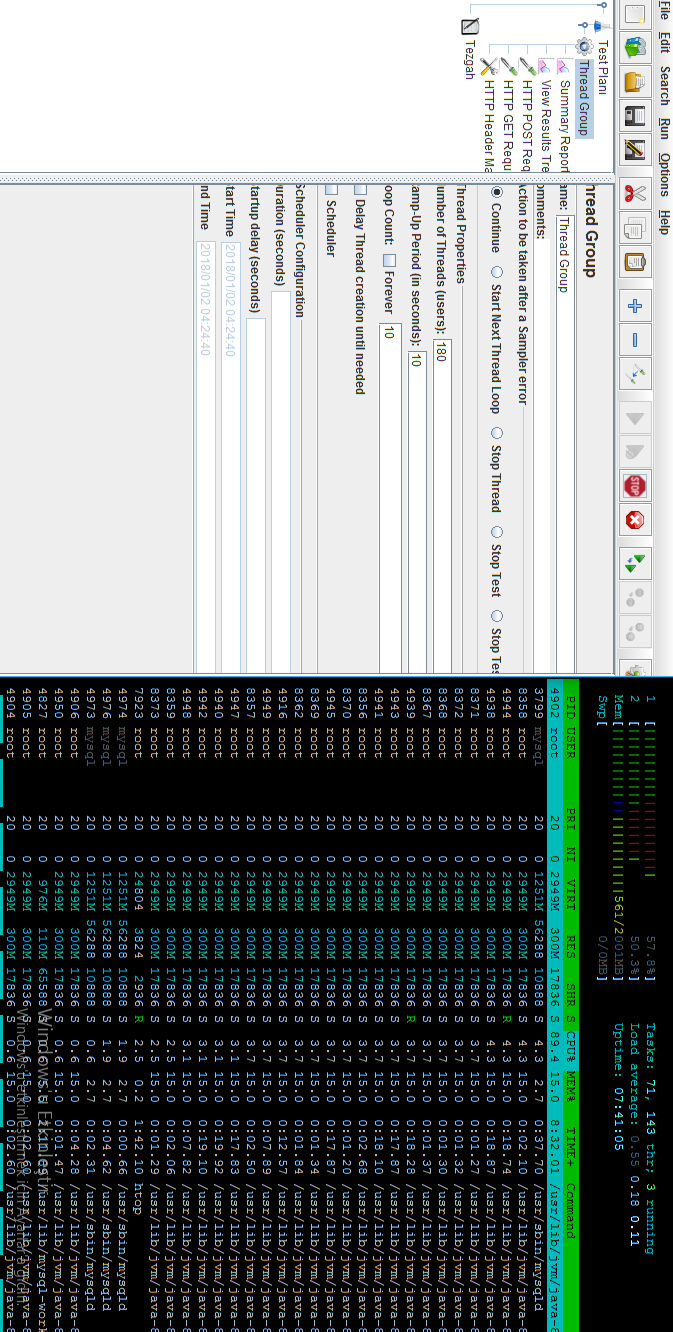
\includegraphics[width=\textwidth]{projectChapters/images/180user.png}
\caption{Server 180 GET and two POST HTTP calls simultaneously}
\label{fig:180user}
\end{figure}


\newpage
 
\subsection{Result}

As we seen the results above, the server can handle up to 200 users simultaneously, its bottleneck is its CPU power, because maximum RAM usage 20 percent even the highest limit of calls.

Comparison between HTTP calls and the result outputs of error rate, throughput, Received KB/sec, Sent KB/sec, Avg Bytes are shown in Figure

\ref{fig:summaryReport}.

\begin{figure}[!htbp]
\centering
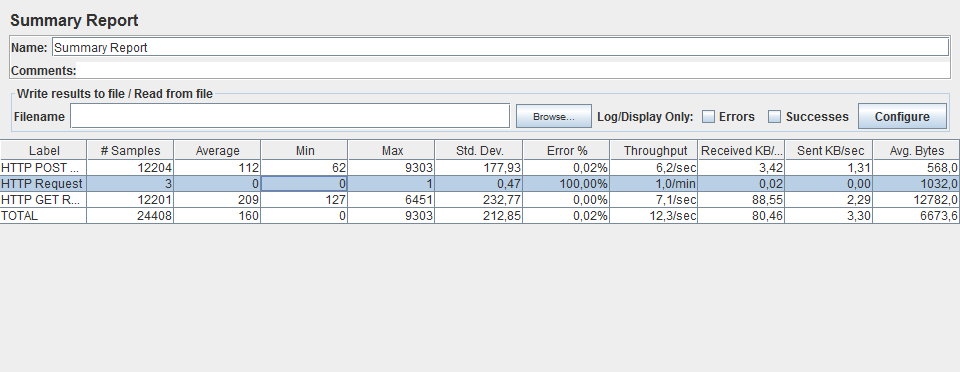
\includegraphics[width=\textwidth]{projectChapters/images/summaryReport.png}
\caption{Summary}
\label{fig:summaryReport}
\end{figure}












